

\section{Results} 
\label{results} 
This section summarizes the key findings of the experiments that were conducted based on the architectures presented in the sections \ref{ensemExp},  \ref{mainExperiments} and \ref{cont_learning_section} of the thesis. Additionally, this section briefly introduces the simplistic UI and evaluates the proposed model on one equipment item from a real plant. 

\subsection{Cross-domain adaptation results}

In order to achieve fair comparison, all experiments obey the following specifications:
\begin{enumerate}
\item The results presented in the subsequent sections will be evaluated predominantly on the T-LESS dataset as introduced in the \nameref{datasets} section. 
\item Thirty objects in the dataset were given arbitrary class names using the following notation: \texttt{Model 1..Model 30}
\item According to the setup defined in Figure \ref{mymodel}, the \underline{teacher model} accepts only the weakly-augmented images from the \underline{target} domain. The primary objective of the model is to improve performance on the target images. Therefore, the primary objective for this ensembled model is to improve the \texttt{AP} on the teacher model. Thus, \texttt{AP50} metrics are recorded for the target images and are then used for comparison. 
\item The base learning rate is defined as \texttt{BASE\textunderscore LR} = 0.001.
\item The number of iterations is fixed at \texttt{MAX\textunderscore ITER} = 50 000.
\item The evaluation happens every \texttt{EVAL\textunderscore PERIOD} = 1000 iterations. Considering that there are 50 000 iterations total, this results in 50 evaluation points across the \texttt{AP50} plot.
\end{enumerate}  

\subsubsection{Scheduler adjustment}
\label{scheduler_section} 
First set of experiments was conducted in accordance with the \nameref{ensemExp} section.  For the baseline comparison, the Adaptive Teacher network was initially trained as it is. This implies that no external components were added and the original learning rate scheduler was used. The pattern of the original scheduler was presented earlier in Figure \ref{annealing} (a). The results of such setup are presented in Figure \ref{original_experiment}. The first graph illustrates the evaluation \texttt{AP50} results for both the teacher and the student models. Although the training process seems idle for the first 20 000 iterations, the model eventually finds better gradients and stabilizes at $max$ (\texttt{AP50}) = 71.40 \% at 31 000 iterations. Even though it might seem that the loss value is decreasing by the end of the training, the \texttt{AP50} value also steadily drops. In order to address the noisy predictions shown earlier in Figure \ref{adapt_experiment1}, the learning rate scheduler has been modified to implement a cosine annealing algorithm without restarts \cite{Loshchilov2016}, as shown in Figure \ref{annealing} (b). The original warm-up period of \texttt{WARMUP\textunderscore ITERS} = 1000 is preserved. 

\begin{figure}[htb]
	\begin{center}
		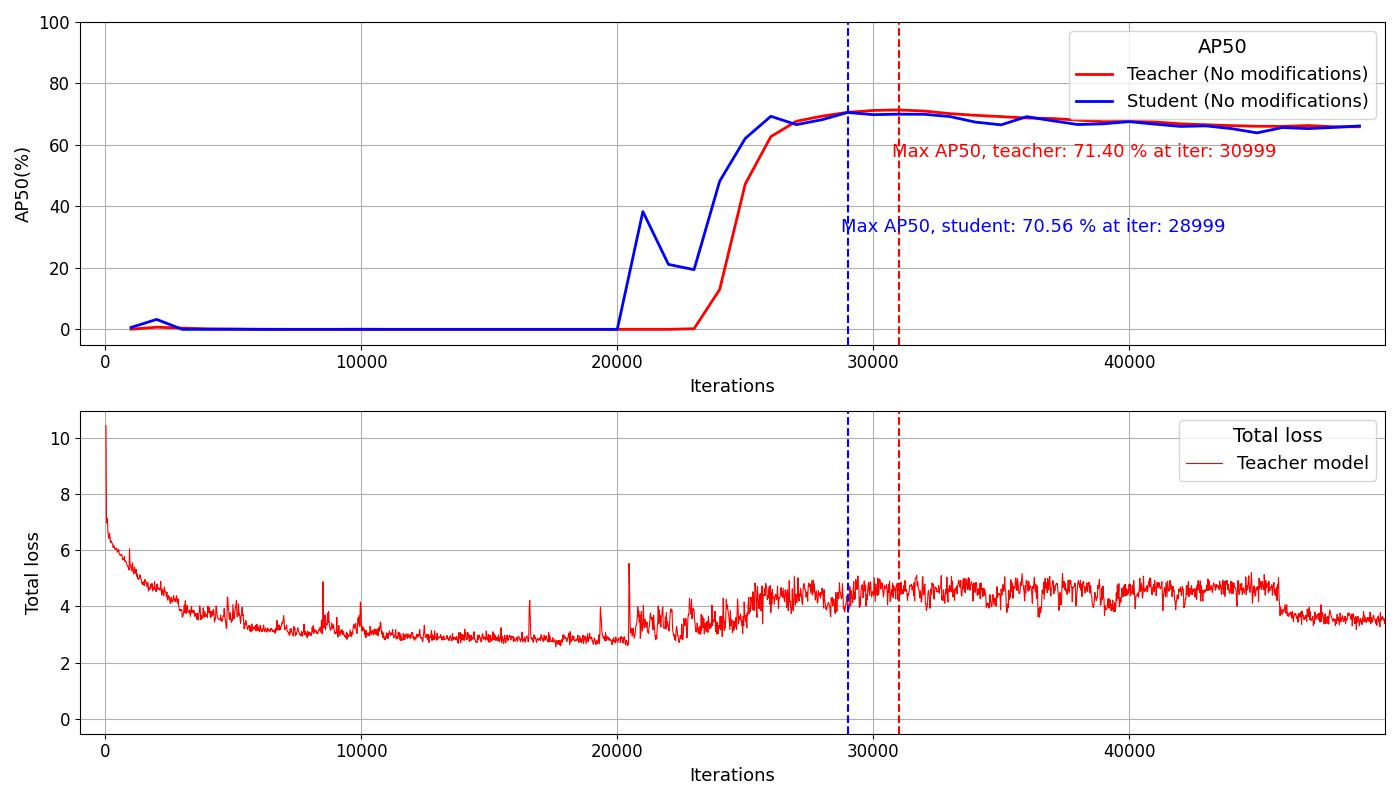
\includegraphics[width=16cm]{./loss&AP50_original.jpg}
	\end{center}
	\caption{Results of the original Adaptive Teacher model evaluated on the custom T-LESS dataset without any modifications.}
	\begin{center}
		\label{original_experiment}
	\end{center}
\end{figure}
Theoretically, this setup would have allowed to find better gradients and reduce overshooting. The results achieved after modifying the scheduler are shown in Figure \ref{comparison_1}. Although the \texttt{AP50} value peaked much faster with the new scheduler, it was only able to reach $max$ (\texttt{AP50}) = 62.50 \%, which is almost 10 \% lower than the original result.   

\begin{figure}[htb]
	\begin{center}
		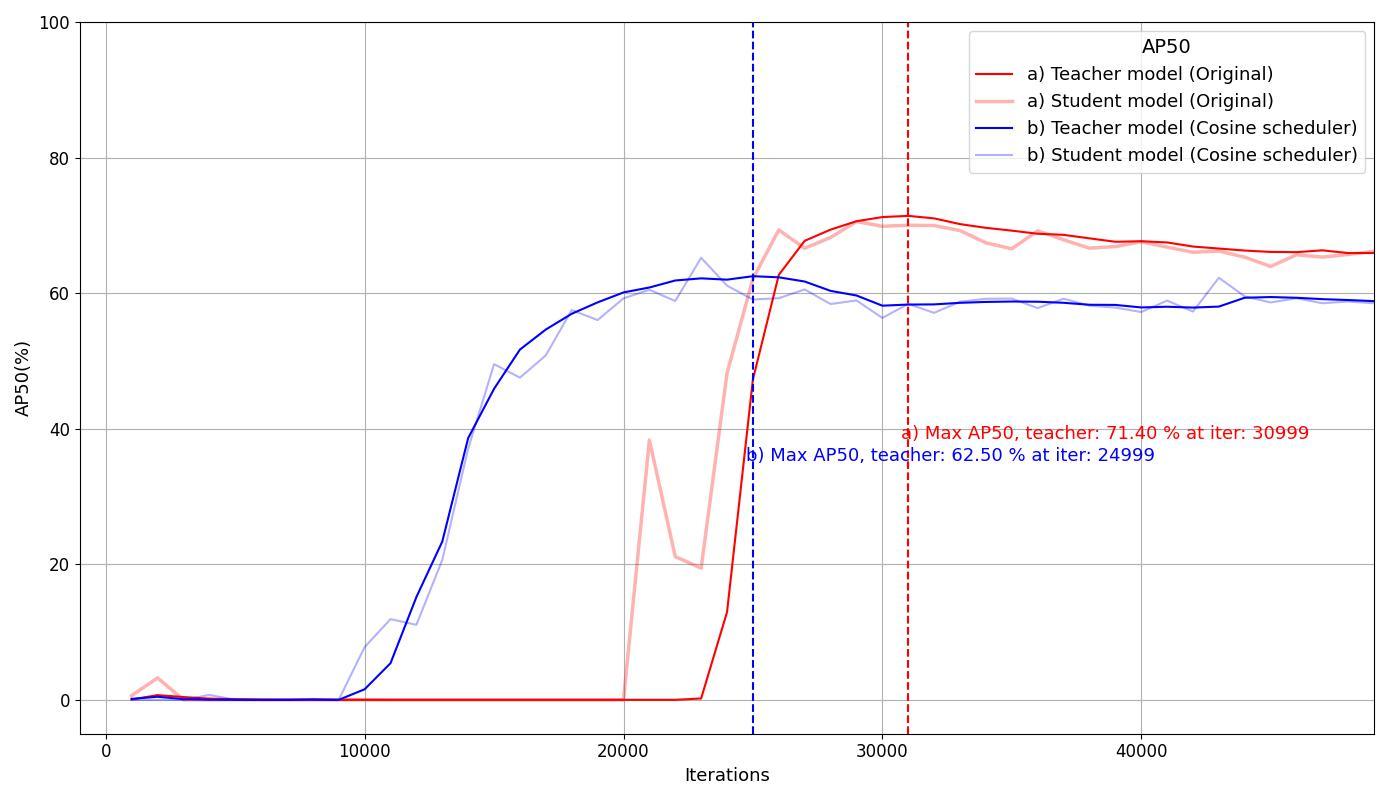
\includegraphics[width=14cm]{./AP50_scheduler.jpg}
	\end{center}
	\caption{a) \texttt{AP50} results of the original model and b) \texttt{AP50} results of the model with a cosine scheduler.}
	\begin{center}
		\label{comparison_1}
	\end{center}
\end{figure}
\FloatBarrier

\subsubsection{Additional augmentations}
\label{augmentations_section} 
Following the ideas proposed in Figure \ref{newAugmentations}, an identical model was trained with two additional strong augmentations. This in theory allows to further diversify the dataset, which will make it less prone to over-fitting. Furthermore, in this and the subsequent  experiments, the model leverages the early stopping algorithm with the parameter of $\texttt{PATIENCE} = 10$. The early stopping algorithm will prevent the model from unnecessary training in case if the \texttt{AP50} does not improve for more than $\texttt{PATIENCE} \times \texttt{EVAL\textunderscore PERIOD} = 10 000$ iterations. The results of the evaluation process with the additional augmentations can be found in Figure \ref{augmentation_experiment}. 
 
\begin{figure}[htb]
	\begin{center}
		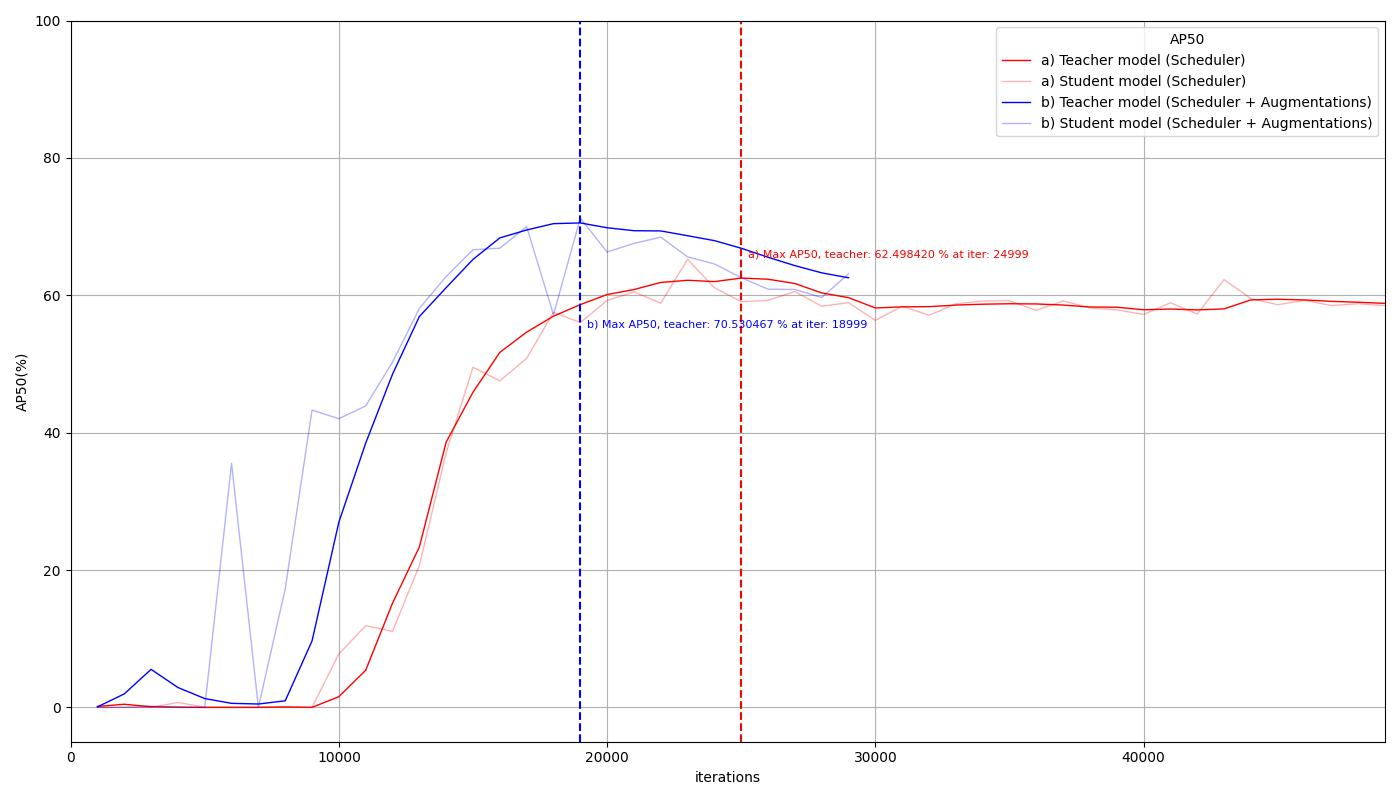
\includegraphics[width=14cm]{./AP50_augmentation.jpg}
	\end{center}
	\caption{a) \texttt{AP50} of the model with a cosine scheduler only and b) \texttt{AP50} results of the model with a cosine scheduler, two additional strong augmentations and the early-stopping algorithm.}
	\begin{center}
		\label{augmentation_experiment}
	\end{center}
\end{figure}

By analyzing these results, it can be easily noticed that the model reaches the peak much faster and the maximum value (\texttt{AP50} = 70.53 \%) is higher than the equivalent model without additional augmentations (\texttt{AP50} = 62.49 \%). Additionally, this model achieves the results, which are competitive to the original Adaptive Teacher implementation (71.40 \%).

\FloatBarrier  

\subsubsection{Instance-level DA and consistency regularization}
The following set of experiments evaluates the custom model presented in Figure \ref{mymodel}. The model utilizes the same principles as in the previous experiment, which includes the cosine scheduler and additional augmentations. On top of it, in this experiment, an instance-level domain adaptation is added along with the consistency regularization term. The regularization weights from Equation \ref{total_loss} are initialized as $\lambda_{\text {consist }} = \lambda_{\text {ins }} = 0.07$. Figure \ref{myModel_experiment} presents the comparison between this model and the model presented in Section \ref{augmentations_section}.

\begin{figure}[htb]
	\begin{center}
		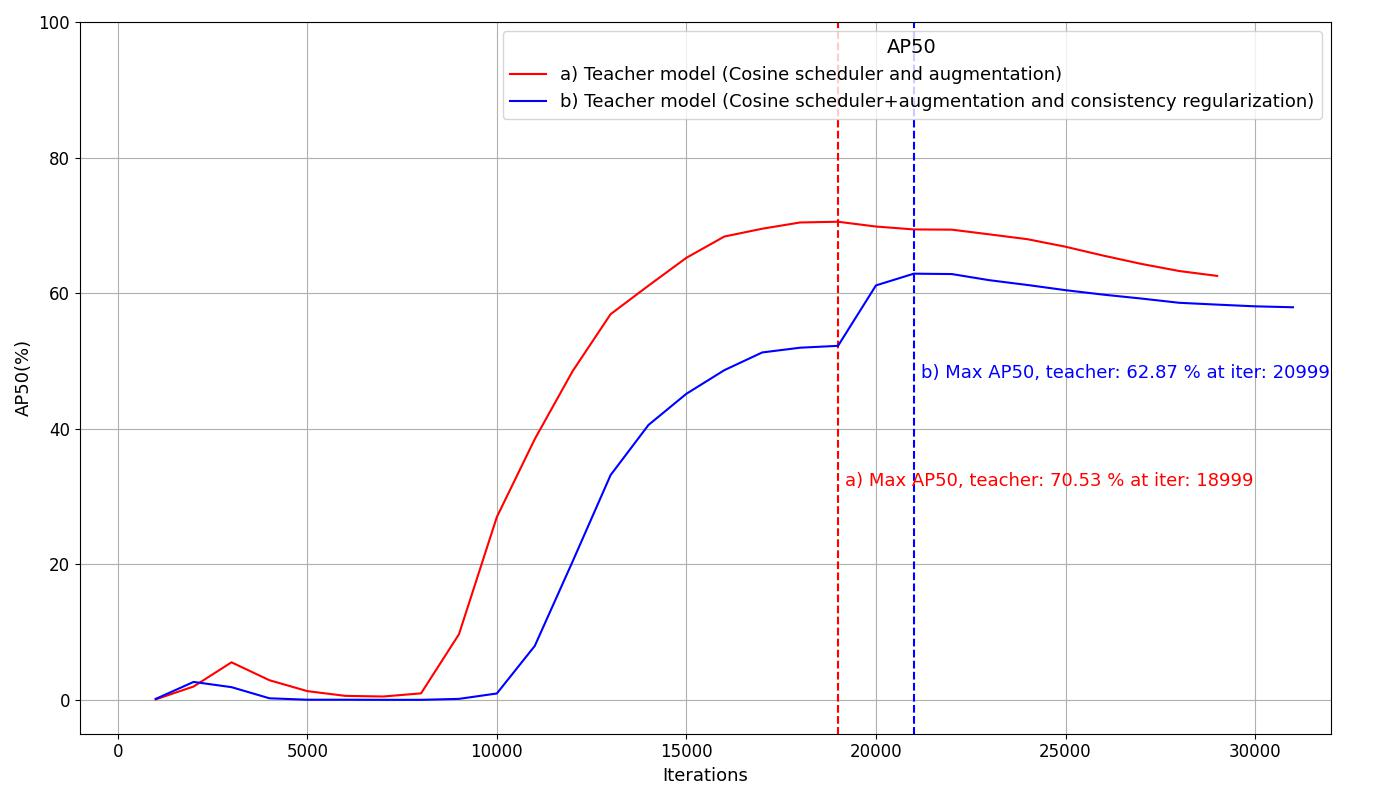
\includegraphics[width=14cm]{./AP50_Augm_consistency.jpg}
	\end{center}
	\caption{a) \texttt{AP50} of the model with a cosine  scheduler and two extra augmentations against b) \texttt{AP50} of the model with a cosine scheduler, two additional augmentations and a consistency regularization.}
	\begin{center}
		\label{myModel_experiment}
	\end{center}
\end{figure}

As it can be concluded, the plot with consistency regularization follows a similar pattern as the pattern in the original model with two custom augmentations. However, the results drop from $max$ (\texttt{AP50}) = 70.53 \% back to  $max$ (\texttt{AP50}) = 62.87 \%. In order to verify the design of the custom components and that they work as intended, an additional experiment was conducted. 

Figure \ref{myModel_constloss_total} illustrates the plots of the instance-level loss and the  consistency loss. As it was defined earlier in the \nameref{mainExperiments} section, the proposed model, similarly as any other adversarial DA model, aims to maximize the instance-level alignment loss in order to confuse the classifier and produce domain invariant features. On the other hand, the model also aims to minimize the consistency loss to force both instance- and image-level classifiers to generate identical outputs for the same image. Although both terms are working as designed, which can be concluded from Figure \ref{myModel_constloss_total}, the \texttt{AP50} value does not improve significantly compared to the original Adaptive Teacher model. 

\begin{figure}[htb]
	\begin{center}
		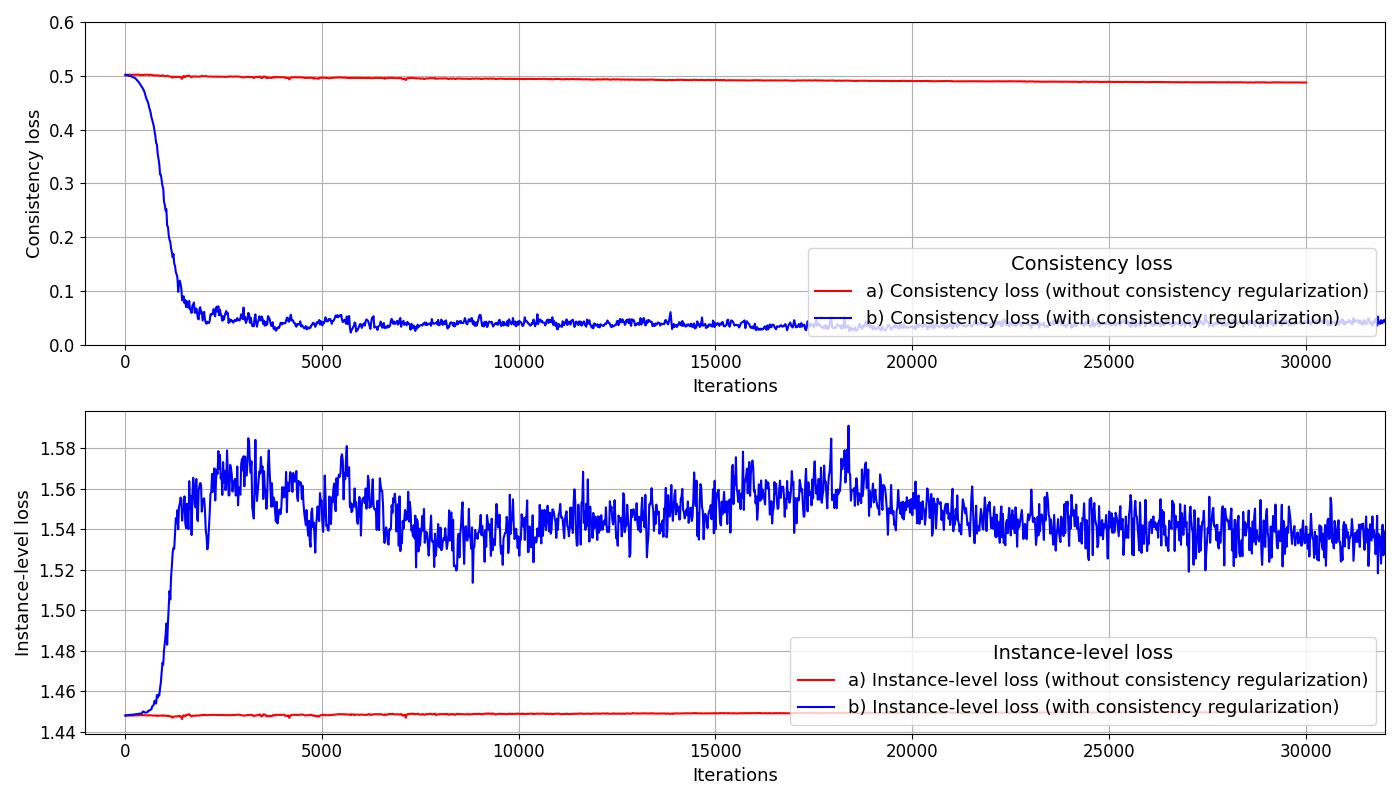
\includegraphics[width=14cm]{./consistency_loss.jpg}
	\end{center}
	\caption{a) The total loss calculation is independent from consistency loss and the instance-level loss terms b) The total loss is proportional to the consistency loss and the instance-level loss terms.}
	\begin{center}
		\label{myModel_constloss_total}
	\end{center}
\end{figure}

A small-scale set of experiments has been additionally carried out in order to identify the optimal weights $\lambda_{\text {consist }}$ and $\lambda_{\text {ins }}$. In order to facilitate the training speed, while preserving fairness in the  comparison process, the maximum number of iterations in all experiments was set as \texttt{MAX\textunderscore ITER} = 30 000. Additionally, to decrease the training time, only the classes 1 to 20 were used for training. The results of six different experiments are shown in Figure \ref{myModel_varying_params}.

\begin{figure}[htb]
	\begin{center}
		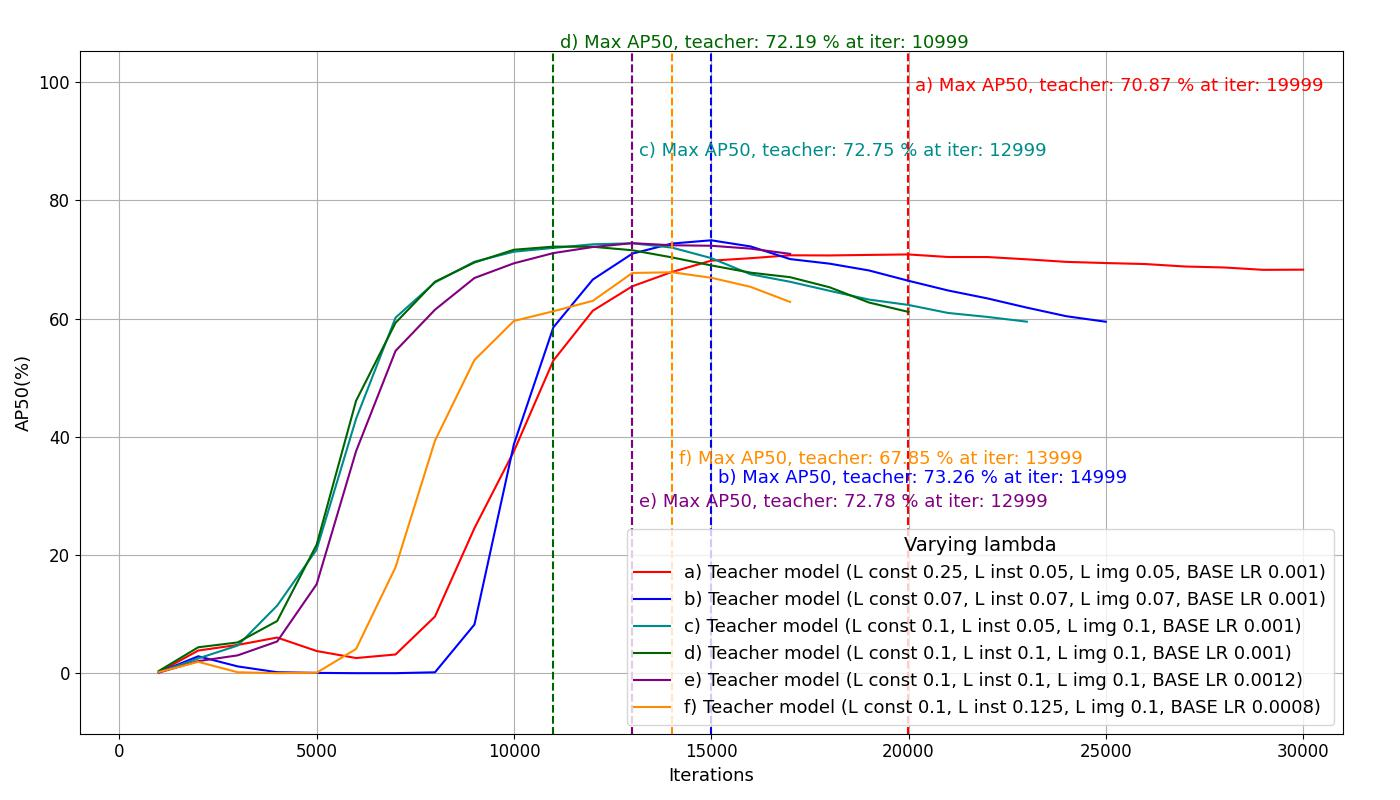
\includegraphics[width=14cm]{./AP50_varying_lambda.jpg}
	\end{center}
	\caption{\texttt{AP50} values for varying weight parameters of $\lambda_{\text {consist }}$, $\lambda_{\text {ins }}$ and \texttt{BASE\textunderscore LR}.}
	\begin{center}
		\label{myModel_varying_params}
	\end{center}
\end{figure}
\FloatBarrier  

From these results, the plot with the $\lambda_{\text {consist }} = 0.07$, $\lambda_{\text {ins }} = 0.07$ and \texttt{BASE\textunderscore LR} = 0.001 were identified to be the best parameters with the resulted \texttt{AP50} = 73.26 \%. However, in practice, more comprehensive experiments should be carried out to determine the best trade-off parameters and the learning rate. 

To verify the performance of the components, one last experiment evaluates the network without the cosine scheduler, which seemed to negatively affect the performance of the subsequent experiments the most (see Figure \ref{comparison_1}). The results of the Regularized Cross-Domain Adaptive Teacher model with the original scheduler are presented in Figure \ref{myModel_withOrigSched}.

\begin{figure}[htb]
	\begin{center}
		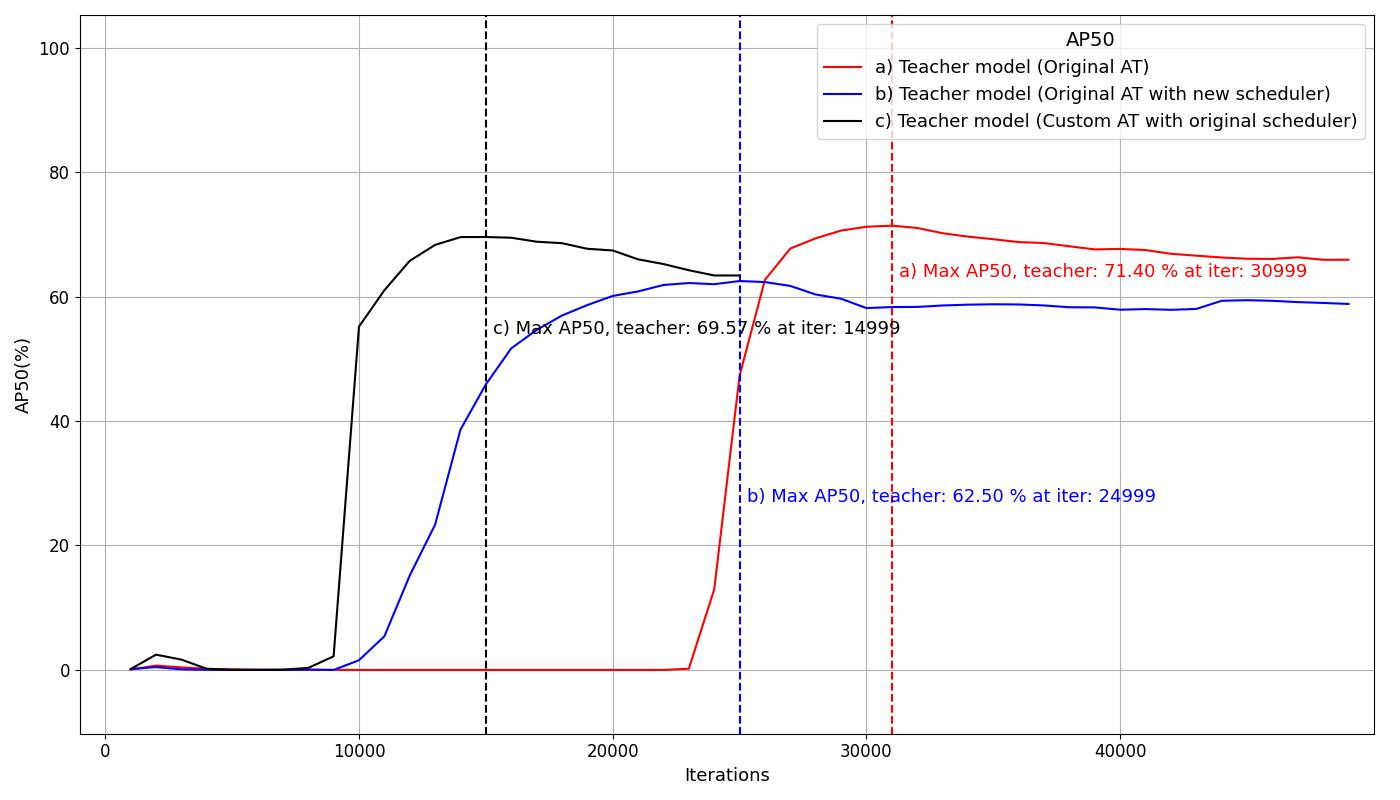
\includegraphics[width=14cm]{./AP50_myModel_origScheduler.jpg}
	\end{center}
	\caption{a) Original model without any modifications b) The custom model with the cosine scheduler c) The custom model with the original scheduler.}
	\begin{center}
		\label{myModel_withOrigSched}
	\end{center}
\end{figure}
\FloatBarrier

According to the results from Figure \ref{myModel_withOrigSched}, the model with consistency regularization, custom augmentations and the default scheduler shows competitive results (\texttt{AP50} = 69.57 \%) compared to the original Adaptive Teacher model (\texttt{AP50} = 70.56 \%, while also peaking significantly earlier (>15 000 iterations faster).  

An additional step has been carried out to verify whether a higher distribution of certain classes affects the model performance (see Figure \ref{tless_distribution_real}). The results of the custom Adaptive teacher model with the original scheduler were filtered and averaged out for the first four classes \texttt{Model 1..Model 4}, which were then compared to the average of the remaining classes \texttt{Model 5..Model 30}. The results can be found in Figure \ref{myModel_withOrigSched_grouped}. 
    
\begin{figure}[htb]
	\begin{center}
	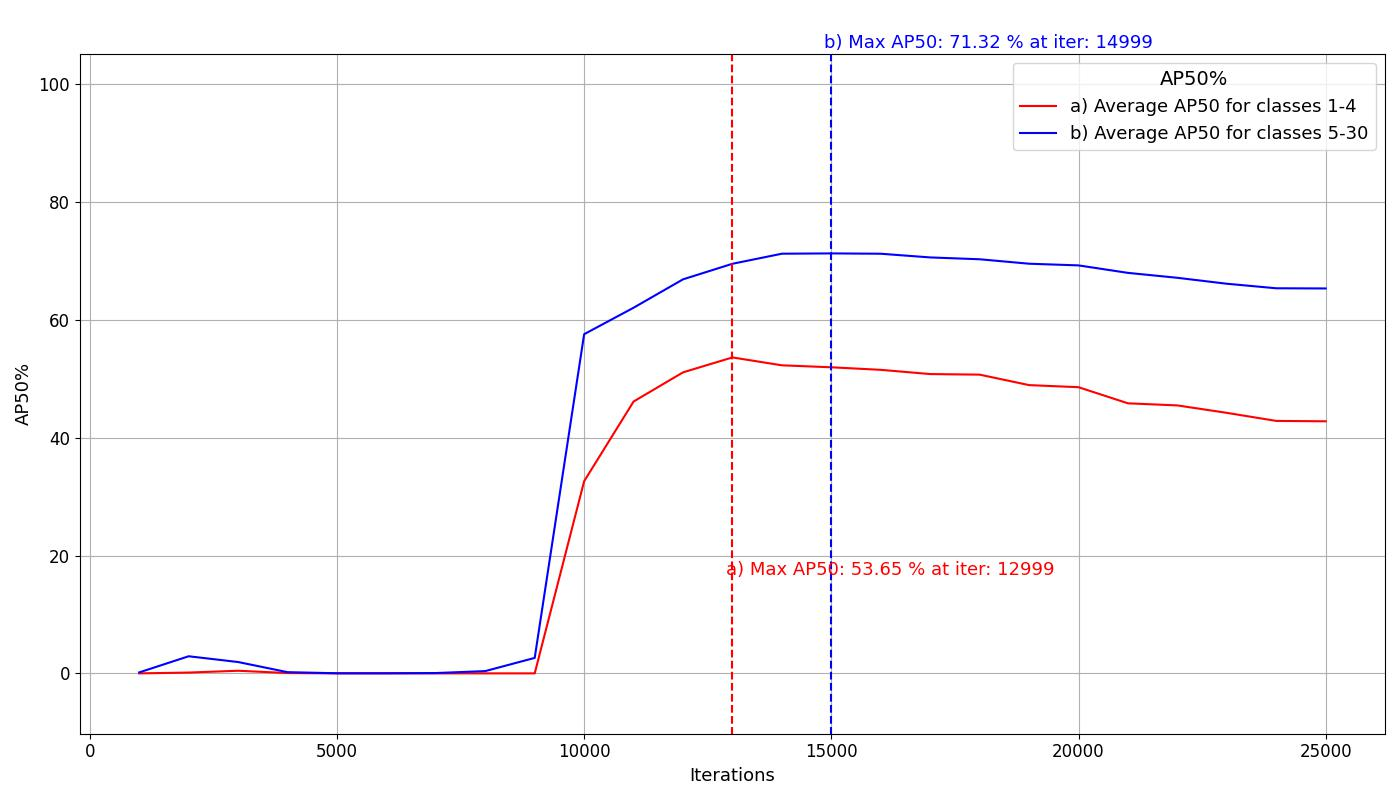
\includegraphics[width=14cm]{./AP50_per_class_group.jpg}
	\end{center}
	\caption{a) Average values of \texttt{AP50} for the classes 1 to 4 b) Average values of \texttt{AP50} for the classes 5 to 30 extracted from the same model results. }
	\begin{center}
	\label{myModel_withOrigSched_grouped}
	\end{center}
\end{figure}

The results of \texttt{AP50} = 53.65 \% for the classes \texttt{Model 1..Model 4} seem to be significantly lower than \texttt{AP50} = 71.32 \% for the remaining classes in the identical setup. This might indicate that higher object distribution in the dataset results in lower detection accuracy as the model struggles to generalize. However, due to a low number of samples, these results might also suggest that the first classes \texttt{Model 1..Model 4} are simply harder to detect. Therefore, more experiments are needed with higher variety in the dataset.  

\subsection{Continual learning results}
\label{cont_learning_results} 
\FloatBarrier 
As was introduced in Figure \ref{tless_distribution_rend}, the entire T-LESS dataset contains 30 different models with objects named arbitrary as \texttt{Model 1..Model 30}. To evaluate the methodology presented in the \nameref{cont_learning_section} section, the following procedure was applied:
 
\begin{enumerate}
\item In the initial experiment, the network was trained on the classes \texttt{Model 1..Model 30}.
\item The second network was only trained on the class \texttt{Model N}, where \texttt{N} is a number between 21 and 30.
\item The third network was trained on the classes \texttt{Model 1..Model 20}.
\item The third network was additionally re-trained to predict the class \texttt{Model N} in a continuous manner from a pre-trained model that was derived in Step 3.
\end{enumerate} 

All networks were based on the model with the cosine annealing scheduler, two custom augmentations and the consistency regularization term. This model was presented earlier in Figure \ref{myModel_experiment}.

Training on the single-class \texttt{Model 21} was selected for the first set of experiments. The results on the class \texttt{Model 21} were filtered out, extracted and, ultimately, the performance was compared between the three suggested methods of training: training from scratch, training individually on one class and training continuously. The combined results for the single class \texttt{Model 21} are presented in Figure \ref{myModel_continuous_experiment_1}.
\FloatBarrier

\begin{figure}[htb]
	\begin{center}
		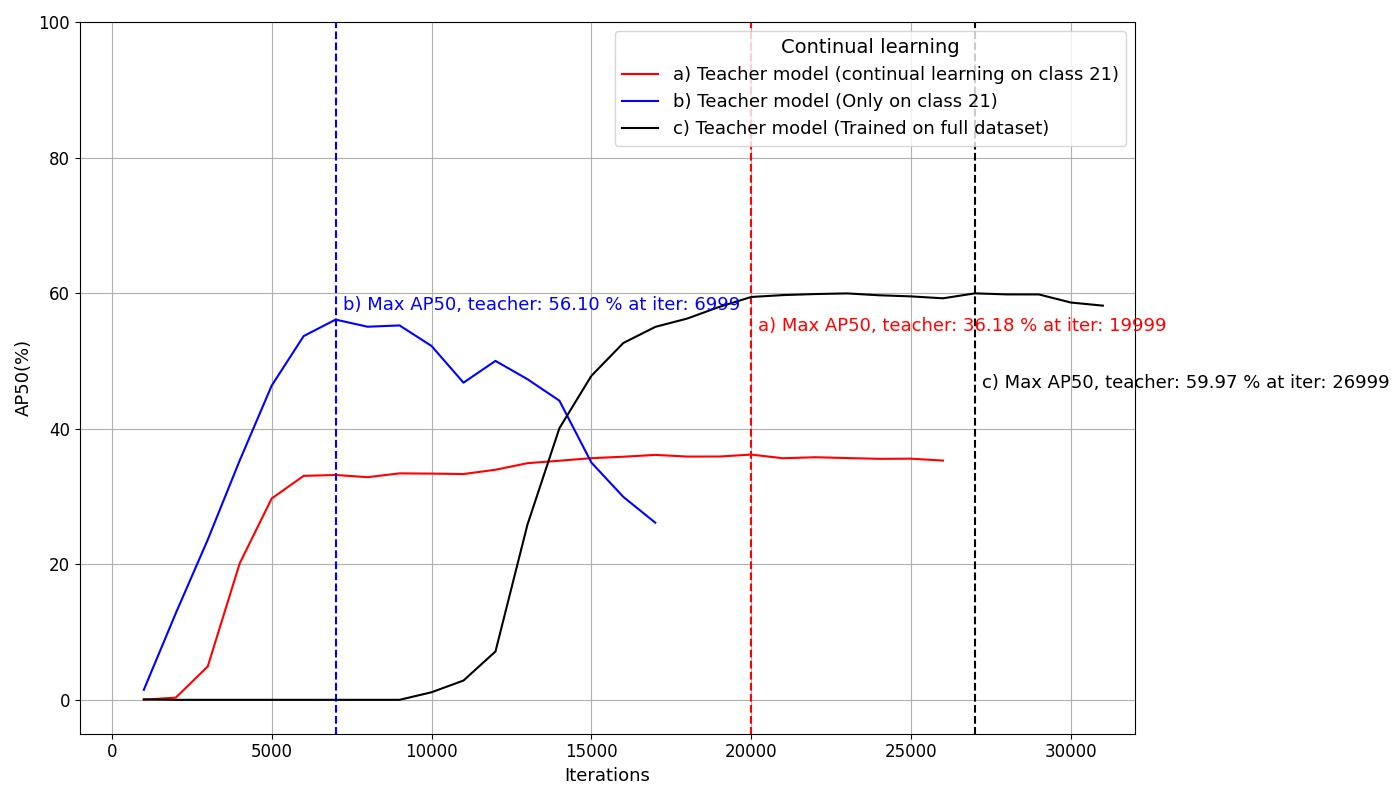
\includegraphics[width=16cm]{./AP50_continual_21.jpg}
	\end{center}
	\caption{The \texttt{AP50} results for class \texttt{Model 21} evaluated in three different setups.}
	\begin{center}
		\label{myModel_continuous_experiment_1}
	\end{center}
\end{figure}

The model trained individually on the \texttt{Model 21} (Figure \ref{myModel_continuous_experiment_1}, a)  rises just as rapidly as it declines. This is contrary to the model trained on the entire dataset (Figure \ref{myModel_continuous_experiment_1}, b), which takes longer to train but also grants better performance on the given class. Meanwhile, the model trained in a continual manner (Figure \ref{myModel_continuous_experiment_1}, c) learns the new class almost just as fast as the model trained purely on the \texttt{Model 21}. However, after a while it stagnates and barely reaches 36\%. 


\begin{figure}[htb]
	\begin{center}
		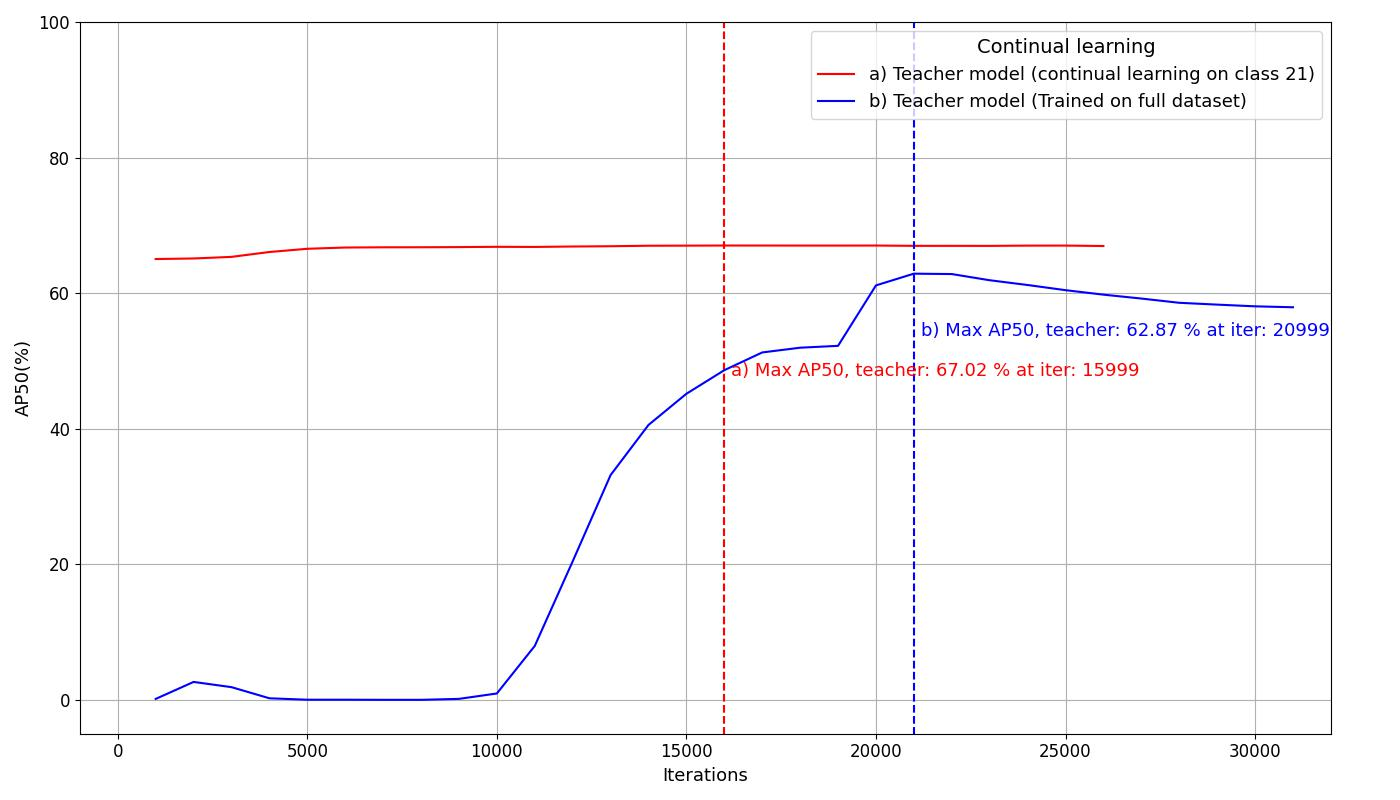
\includegraphics[width=14cm]{./AP50_continual_21_allClasses.jpg}
	\end{center}
	\caption{a) The total \texttt{AP50} value evaluated on the classes \texttt{Model 1..Model 21} using continual learning b) The total \texttt{AP50} results for the classes \texttt{Model 1..Model 30} on the model that was trained from scratch.}
	\begin{center}
	\label{myModel_continuous_experiment_0}
	\end{center}
\end{figure}
\FloatBarrier

The average continual learning results of the total \texttt{AP50} for classes \texttt{Model 1..Model 21} (Step 4) were also compared to the average total \texttt{AP50} results for classes \texttt{Model 1..Model 21} when trained from scratch (Step 1). This comparison is presented in Figure \ref{myModel_continuous_experiment_0}. According to this plot, the overall \texttt{AP50} trend seems to be increasing, which means that the model is slowly learning new data without losing the previously obtained knowledge, thus solving the catastrophic forgetting problem. 

The plots follow similar patterns when repeating the training steps for other classes of objects. The results can be found in Figure \ref{myModel_continuous_experiment_2}.

\begin{figure}[htb]
	\begin{center}
		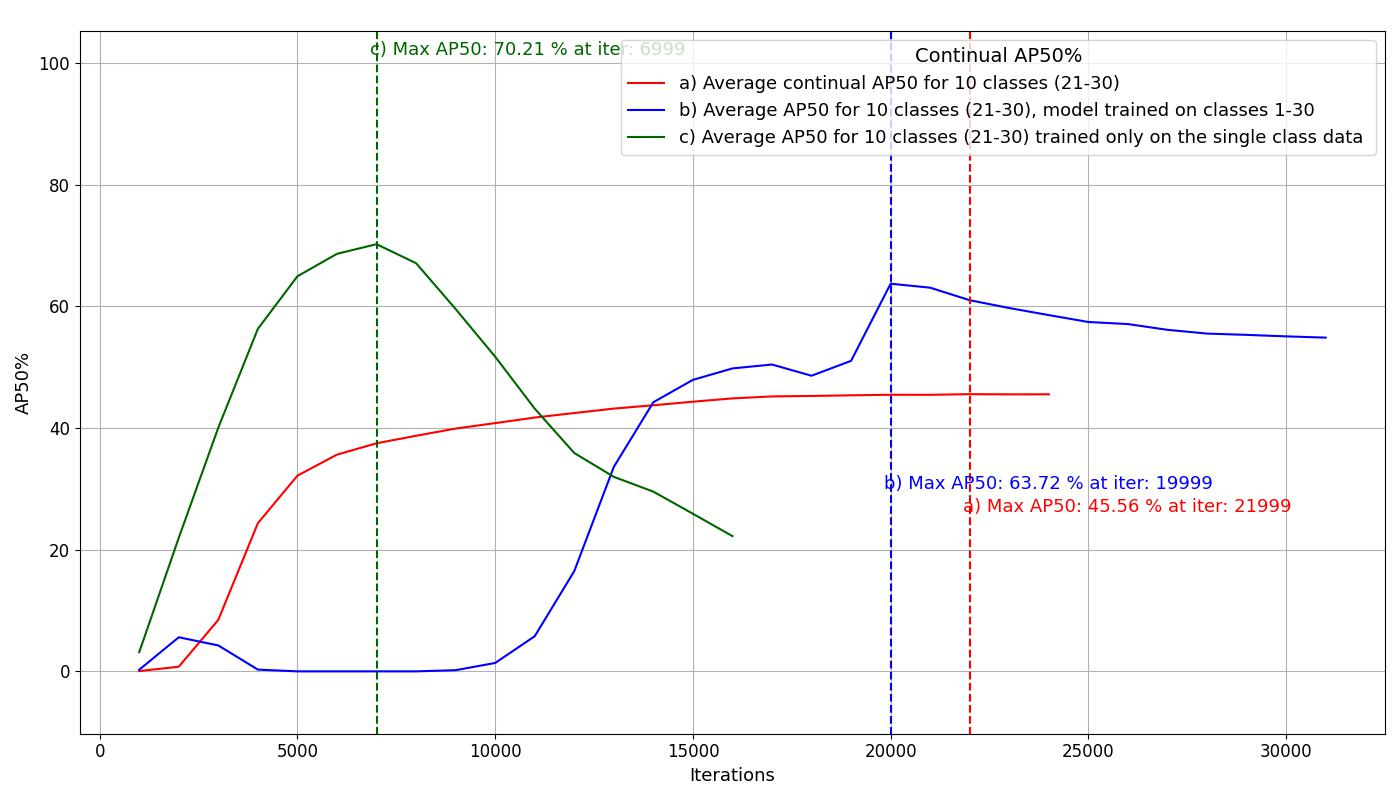
\includegraphics[width=14cm]{./continualAP_average_21to30.jpg}
	\end{center}
	\caption{a) The average \texttt{AP50} value for continual learning on classes \texttt{Model 21..Model 30} given the model trained on classes \texttt{Model 1..Model 20}  b) The average \texttt{AP50} value for classes \texttt{Model 21..Model 30} extracted from the original model trained from scratch on classes \texttt{Model 1..Model 30} c)  The \texttt{AP50} value for each of the classes \texttt{Model 21..Model 30} when trained individually. The values are then averaged out for all 10 classes.}
	\begin{center}	\label{myModel_continuous_experiment_2}
	\end{center}
\end{figure}
\FloatBarrier

  
Here, Step 4 was repeated for the classes \texttt{Model 21..Model 30} based on the model derived from Step 2. Consequently, the average of the mean results for each of the classes were combined to form the plot in Figure \ref{myModel_continuous_experiment_2} (a). For  comparison, the training results for the classes \texttt{Model 21..Model 30} were extracted from the results of the training on the entire dataset (Step 1). Such plot is illustrated in Figure \ref{myModel_continuous_experiment_2} (b). Finally, Figure \ref{myModel_continuous_experiment_2} (c) illustrates the \texttt{AP50} value for the average of each of the classes \texttt{Model 21..Model 30} when trained individually (Step 2). 

As it can be concluded, training the model on each of the classes individually yields the best results \texttt{AP50} = 70.21 \%. Additionally, it can be noted that the model achieves a higher \texttt{AP50} when trained from the scratch (\texttt{AP50} = 63.672\%), compared to the model trained continuously, which saturates at the much lower value of \texttt{AP50} = 43.56\%. However, it takes considerably less time to train the model continuously, as this lifelong learning model reaches 90 \% of its maximum \texttt{AP50} value already in about 7000 iterations.


To conclude, the presented continual learning approach has proven to be able to learn new classes. Despite being less efficient that training the model from scratch, it adequately solves the catastrophic forgetting problem, which was discussed earlier in Section \ref{cont_learning}.

\FloatBarrier
\clearpage
\subsection{Deployment results}
\FloatBarrier
In order to showcase the performance of the proposed model, a simple web app was developed. The app was hosted on a local server and it leverages Flask API to connect the detector app to the user interface. The app utilizes the model, which was presented in Figure \ref{myModel_withOrigSched} due to its relatively good performance and the fastest training speed among the competitors. The prototype of the UI is presented in Figure \ref{demo}. 

\begin{figure}[htb]
	\begin{center}
		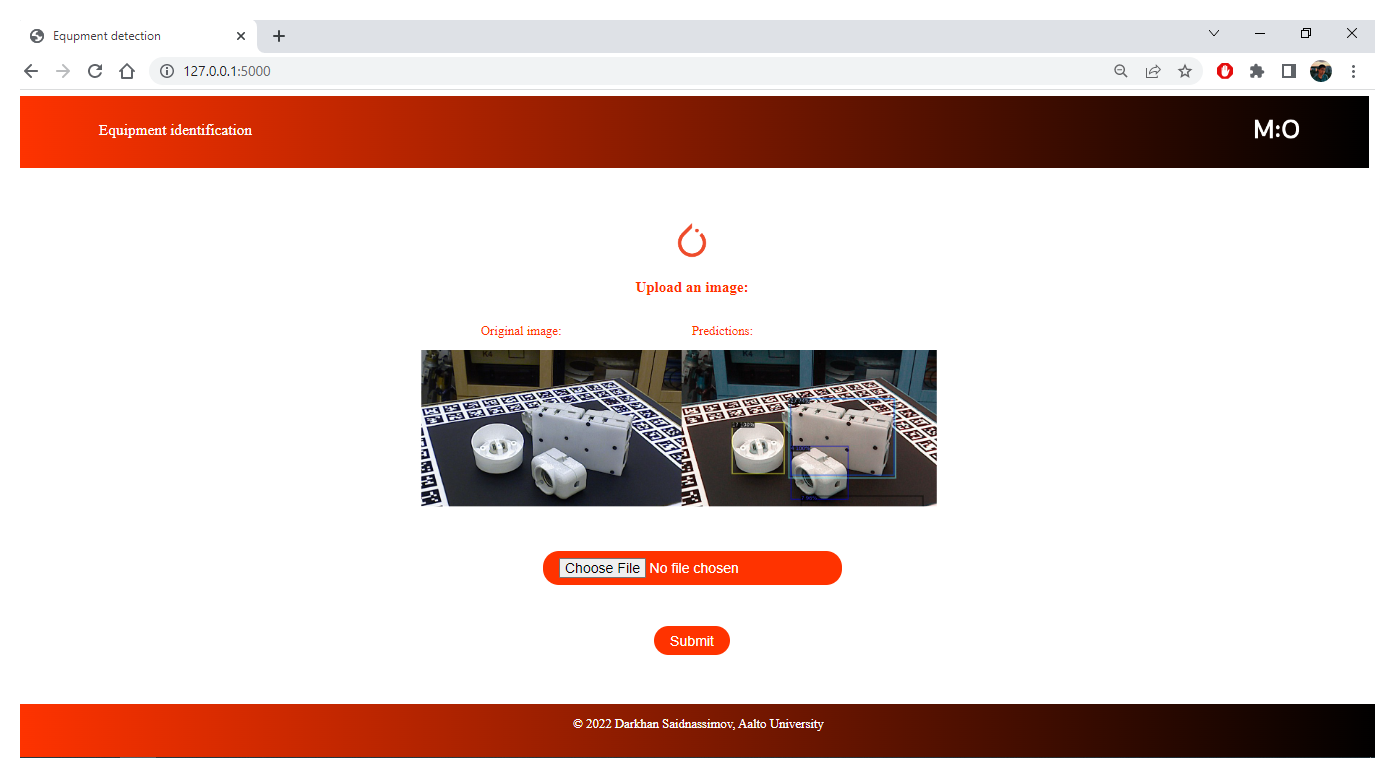
\includegraphics[width=14cm]{./demo.png}
	\end{center}
	\caption{A screenshot of the simple web app. The image on the left-hand side represents an uploaded target image with the objects to predict, and the image on the right-hand side returns the localized objects.}
	\begin{center}
		\label{demo}
	\end{center}
\end{figure}

The app sends \texttt{POST} requests to upload an image to localhost via Flask API. The uploaded image is forwarded as an input to the model and returned to the user interface along with the predictions (if any) after running the inference on the CPU node. Loading an image to the model takes about 0.0012 s, while running the inference on the image takes about 0.0466 s. However, the uploading time is essentially the bottleneck of the detection process as it would vary depending on the internet connection speed and whether the server is located on the localhost or not. 

The complete app is built using Python 3.9, while the model additionally utilizes packages and frameworks such as Pytorch 1.10.1, CUDA 11.3 and Detectron2 v0.6. The model was trained on Nvidia A100 units. The hardware and the computing resources were provided by CSC - Finnish IT Center for Science. 


\FloatBarrier

\clearpage

\subsection{Evaluation on the real equipment}
\label{real_equipment_tests} 
In the final set of experiments, the proposed model was briefly evaluated on the real equipment. As discussed in the \nameref{datasets} section, the rendered images of the equipment can be obtained from the 3D CAD models. Although the images can be rendered using a script that would automatically rotate around the object in 3D-plane and save the images, for the purpose of this experiment, the rotation around the object was performed manually and the video recording of the operation was saved. Then, the recording was split into frames and 1 000 images of an industrial \texttt{HM-75S} pump were collected. These images were then labeled using LabelImg \cite{2015} annotation tool as illustrated in Figure \ref{Fig:rendered_pump}. This subset of images will act as a source domain and is used only for training. 

On the other hand, a handful of 28 real \texttt{HM-75S} pump images were collected from the plant. An example image is shown in Figure \ref{Fig:real_pump}. These real images will act as a target domain and the main objective of this experiment is to identify and localize the real images of the pump correctly. 

\begin{figure}[!htb]
   \begin{minipage}{0.45\textwidth}
        \centering
     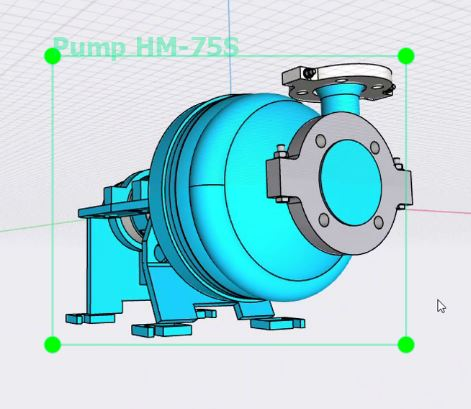
\includegraphics[width=0.9\linewidth]{./annotation_process.jpg}
     \caption{Labeled image of the rendered \texttt{HM-75S} pump}\label{Fig:rendered_pump} 
   \end{minipage}\hfill
   \begin{minipage}{0.45\textwidth}
\centering
     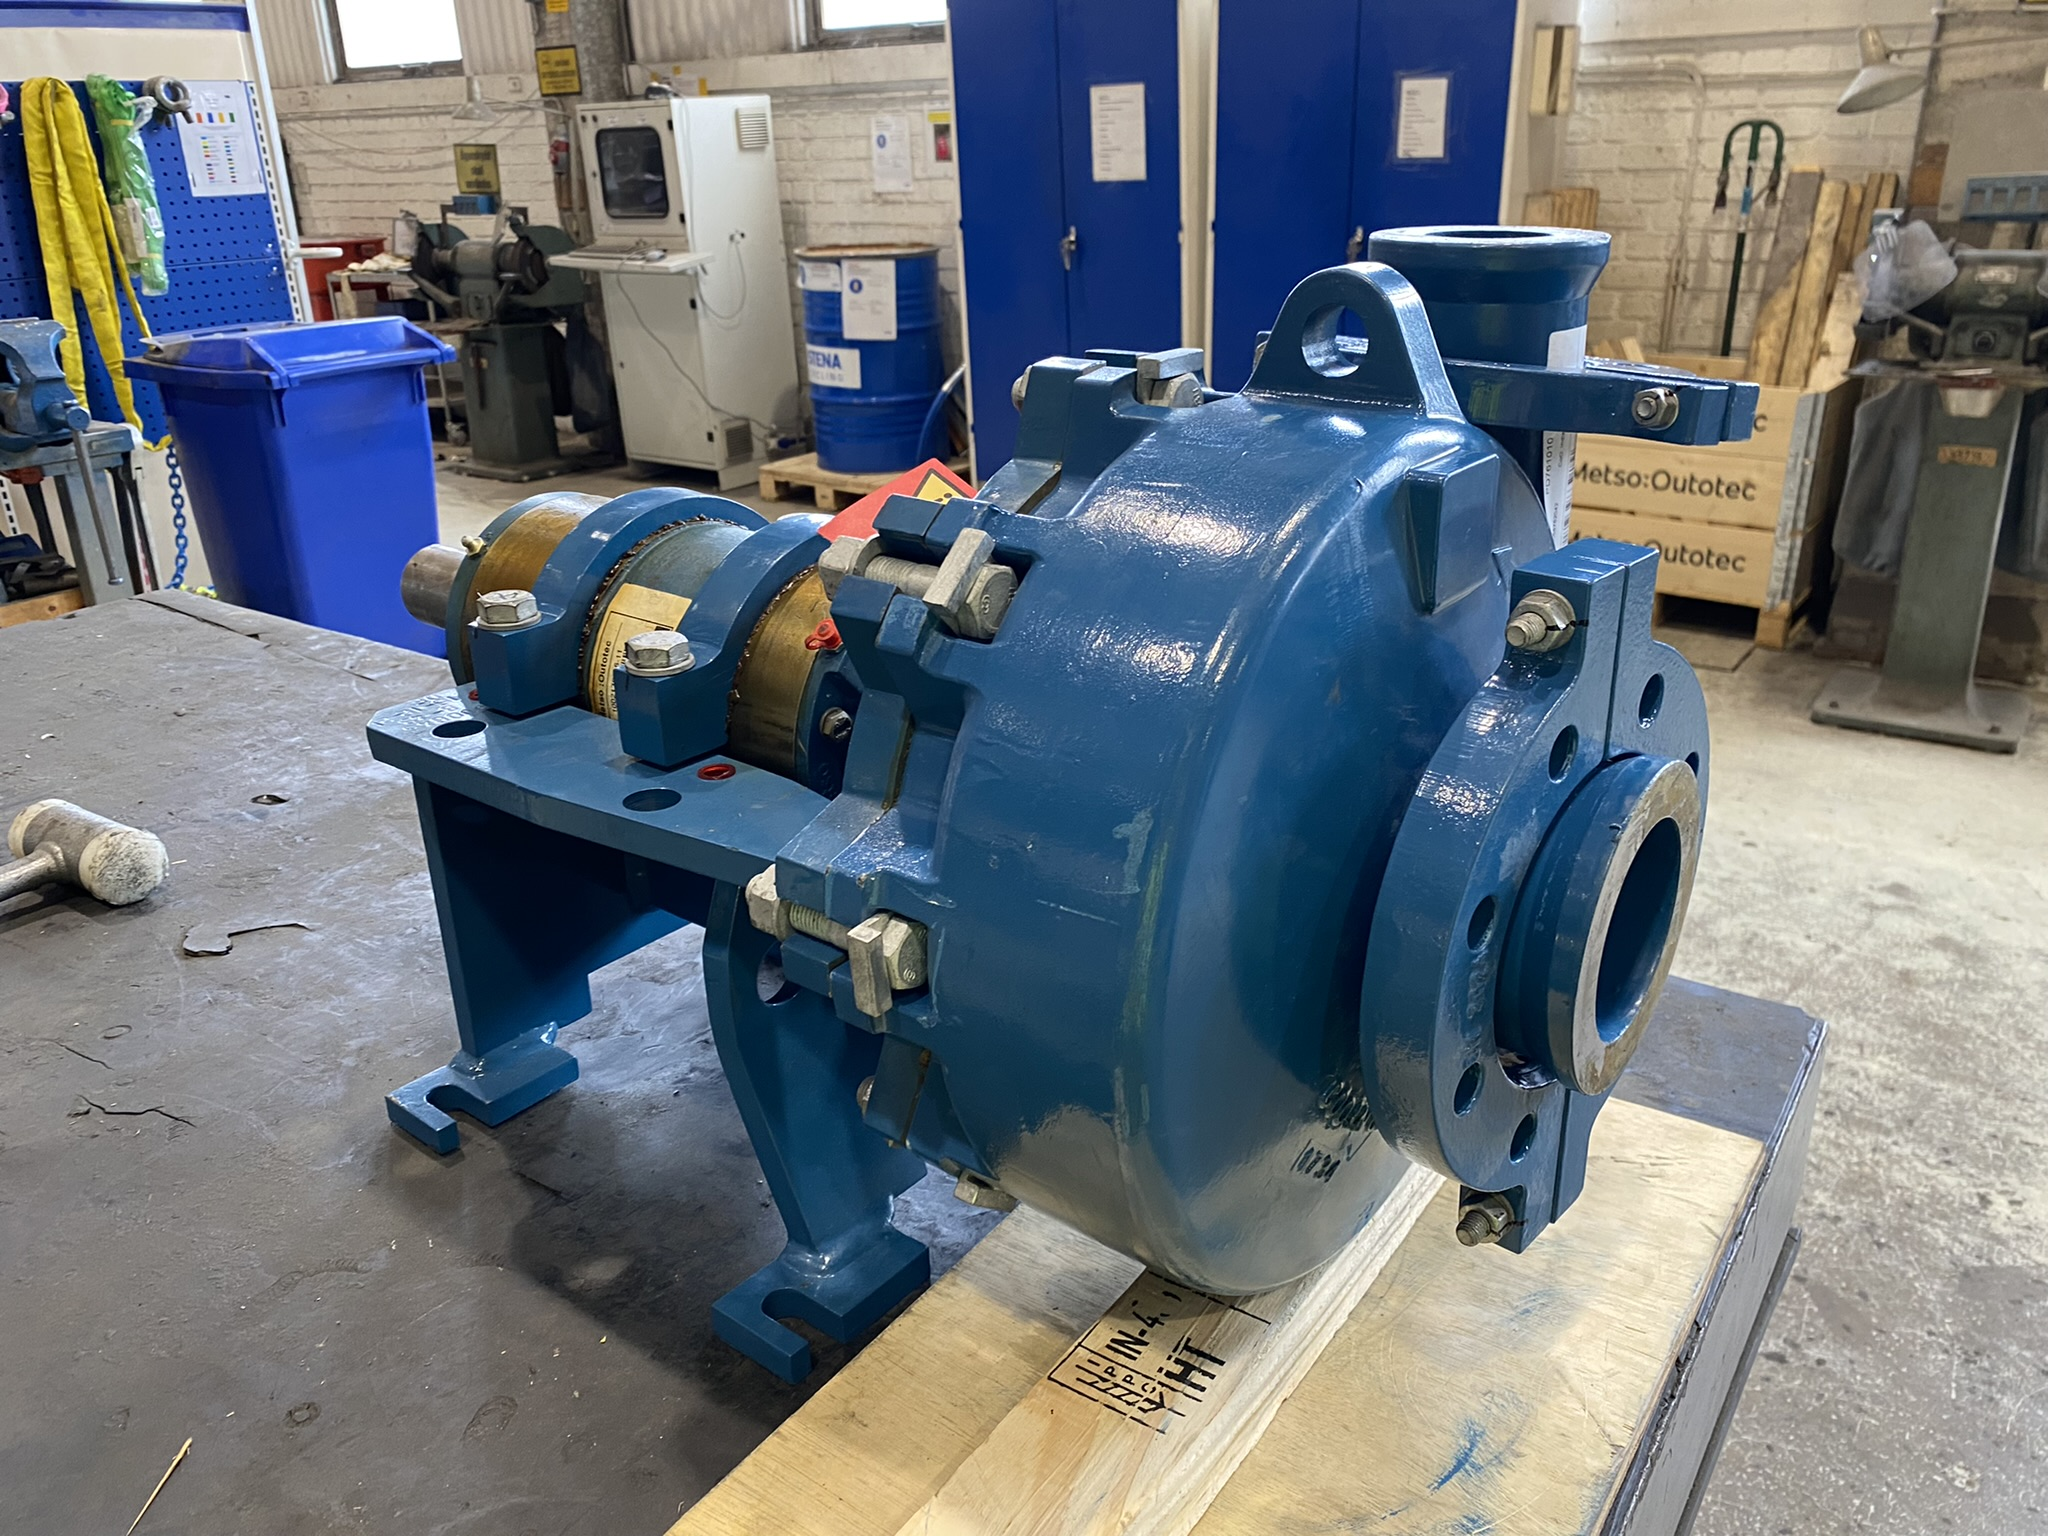
\includegraphics[width=\linewidth]{./pump_real.jpg}
     \caption{Unlabeled image of the real \texttt{HM-75S} pump}\label{Fig:real_pump}
   \end{minipage}
\end{figure}

In theory, these images do not require labeling. However, as it was defined in the \nameref{datasets} section, the target dataset is split into two subsets for training and for testing. This in practice means that in order to evaluate the model and to compare the results, the testing subset must be labeled. For this experiment, the splitting ratio was selected to be 70 \% to 30 \% for the training and testing subsets, instead of the originally proposed ratio of 85 \% to 15 \%. The number of the testing images was essentially increased to account for the target dataset of a fairly limited size. This resulted in 19 training and 9 testing images of the real pump. 

The entire training dataset (1000 rendered and 19 real images) was then forwarded to the Adaptive Teacher model with consistency regularization and the original scheduler (see Figure \ref{myModel_withOrigSched}). The training conditions were identical as in the previous experiments and the obtained results are shown in Figure \ref{pump_results}. 

\begin{figure}[htb]
	\begin{center}
		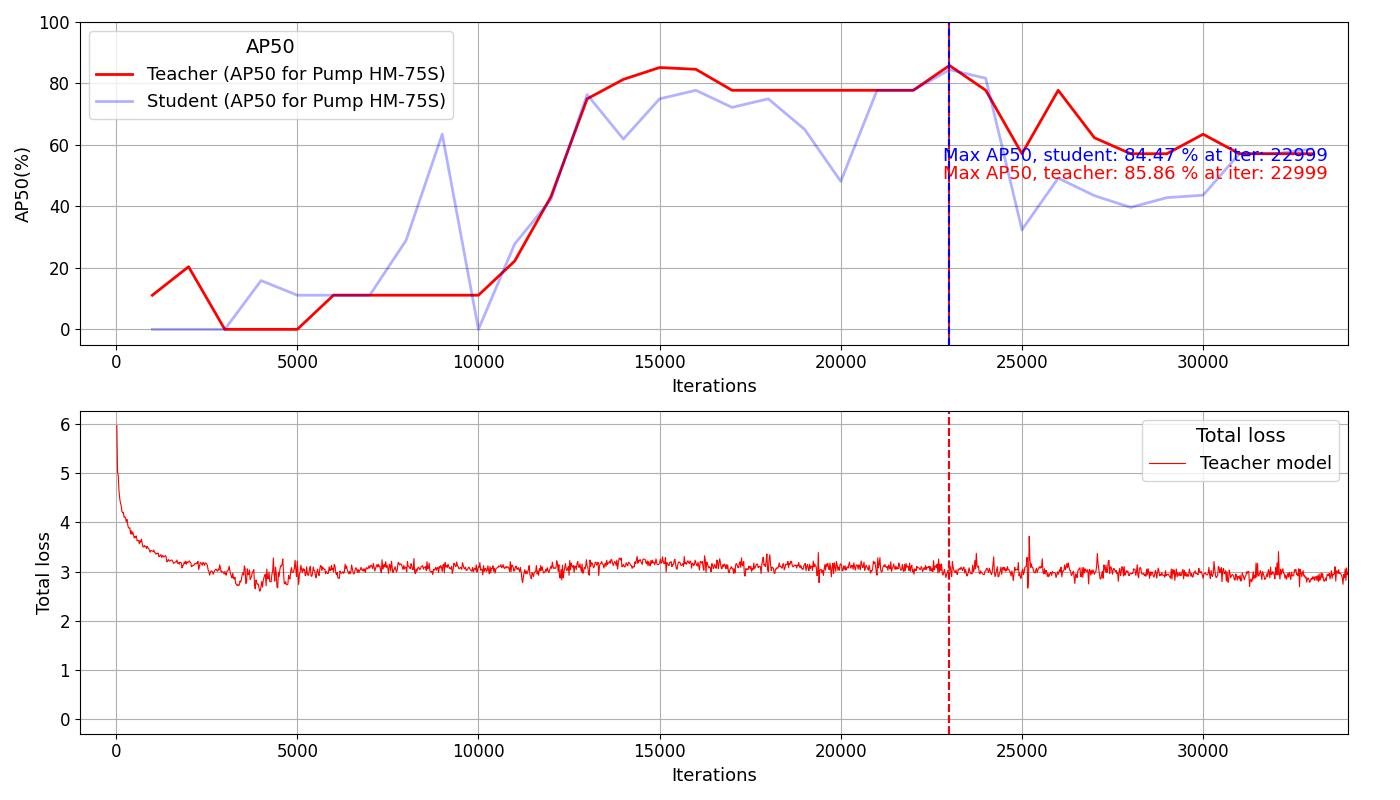
\includegraphics[width=14cm]{./loss&AP50_pump.jpg}
	\end{center}
	\caption{The performance of the proposed model on the custom dataset with one industrial object.}
	\begin{center}\label{pump_results}
	\end{center}
\end{figure}
\FloatBarrier

The results suggest that the model performance starts improving at 10 000 iterations, similarly to the earlier experiments (see Figure \ref{myModel_withOrigSched}). The best \texttt{AP50} result of 85.86 \% is achieved at 22 999 iterations. Finally, the model was deployed to the simplistic web app and the results of the prediction are visualized in Figure \ref{pump_demo}.


\begin{figure}[htb]
	\begin{center}
		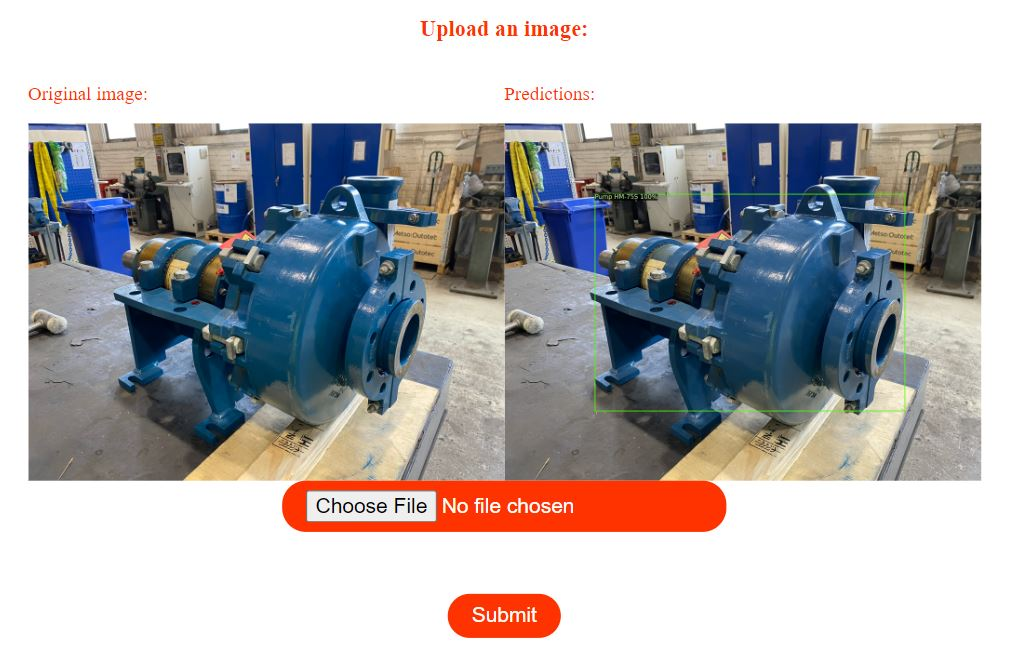
\includegraphics[width=16cm]{./pump_demo.jpg}
	\end{center}
	\caption{The demonstration of the model that was trained on the source and target images of the \texttt{HM-75S} pump. The model correctly identifies a pump in the real environment. }
	\begin{center}\label{pump_demo}
	\end{center}
\end{figure}
\FloatBarrier

Although the model seems to show a relatively good performance on the target dataset and correctly identifies the pump in the given images, this experiment was carried out to showcase the applicability of the method on the real-life industrial datasets, rather than to extensively evaluate the performance. In reality, a dataset of 28 real images is rather insufficient and a larger target dataset must be collected in order to produce more practical results. 


\clearpage

